%! Author = gramic
%! Date = 19.03.24

% Preamble
\begin{flushleft}
    \subsubsection{Sharding}
    \paragraph{Vertikales / Horizontales Sharding}
    Tabellen können Horizontal oder Vertikal partitioniert werden.
    \begin{figure}[H]
        \centering
        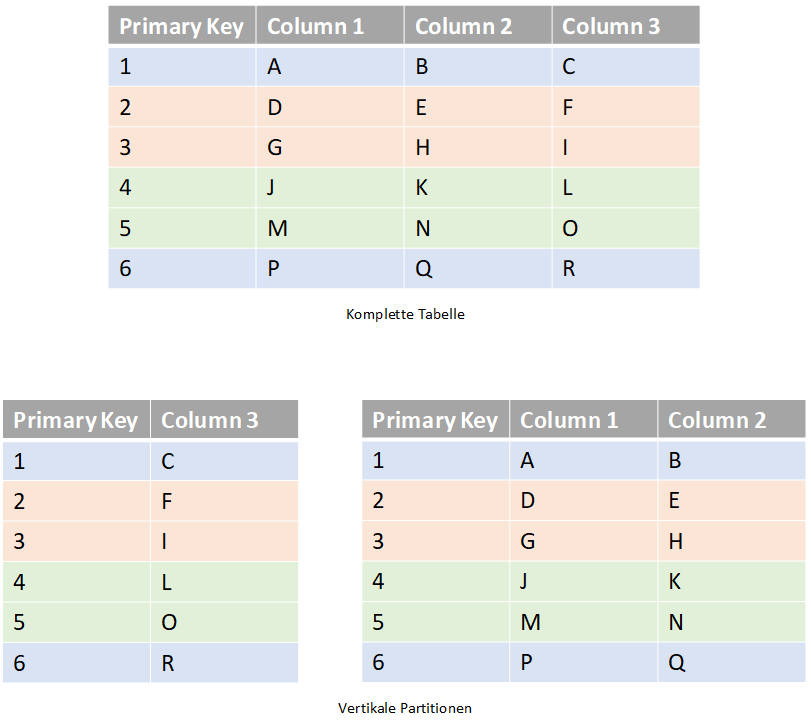
\includegraphics[width=0.8\linewidth]{source/implementation/evaluation/excursus_architecture/sharding_vertical_partitioning}
        \caption{Sharding - Vertikale Partitionierung}
        \label{fig:sharding_vertical_partitioning}
    \end{figure}
    \begin{figure}[H]
        \centering
        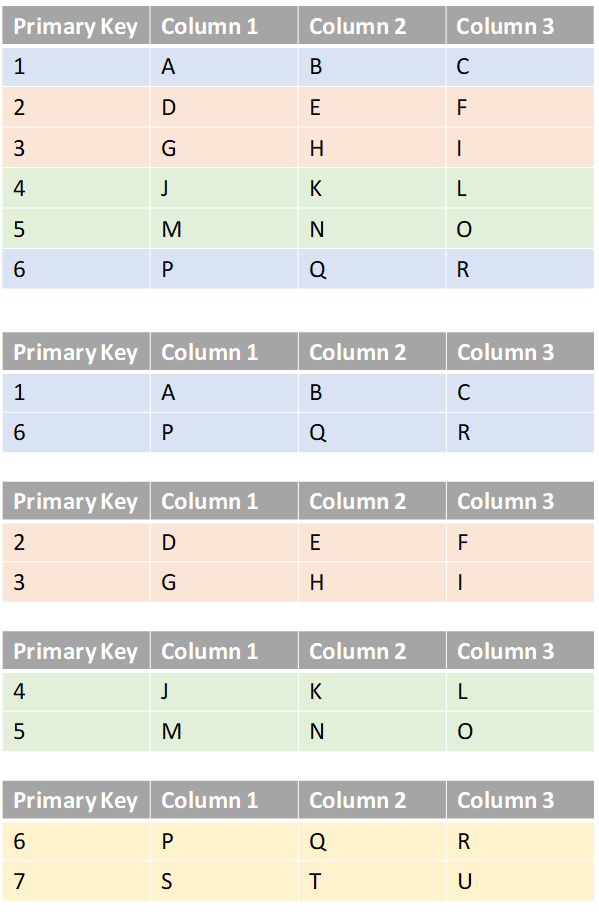
\includegraphics[width=0.8\linewidth]{source/implementation/evaluation/excursus_architecture/sharding_horizontal_partitioning}
        \caption{Sharding - Horizontales Partitionierung}
        \label{fig:sharding_horizontal_partitioning}
    \end{figure}
    Horizontales Partitionieren wird meistens für das Sharding von Tabellen benutzt.
    Die Partitionen entsprechen dann den Shards.
\begin{flushleft}
\end{flushleft}
    \paragraph{Key Based Sharding}
    Hierbei wird das sharding anhand eines oder mehreren Keys ausgeführt.
\begin{flushleft}
\end{flushleft}
    \paragraph{Range Based Sharding}
    Das Sharding wird dabei anhand von Ranges ausgeführt.
    Zum Beispiel anhand von Preis-Ranges.
\begin{flushleft}
\end{flushleft}
    \paragraph{Directory Based Sharding}
    Hierfür wird eine lookup-Tabelle geführt, welche die Schlüssel für das Sharding bereitstellen.
    Anhand dieser werden dann die entsprechenden Zieltabellen aufgeteilt.
\begin{flushleft}
\end{flushleft}
    \paragraph{Hash Based Sharding}
    Das Hash Based Sharding ist eine Form des Range Based Shardings, bei dem Hashwerte der Datensätze benutzt werden.
    Je nach Bereich wird der Datensatz dann einem Shard zugewiesen.
\end{flushleft}